\chapter{Zeitplanung}
Die Initiale Zeitplanung wurde in jedem Iterationmeeting besprochen und entsprechend nachgeführt. Nachfolgend ist die Entwicklung der Planung zu sehen. Diese Nachführung hat den Zweck allfällige Abweichungen frühzeitig zu erkennen und entsprechend schnell reagieren zu können. Wöchentliche Iterationsmeetings im Entwicklungsteam intern und wöchentliche Statusmeetings mit Herrn Steffen \& Brunner stellen sicher, allfällig auftretende Komplikationen frühzeit zu erkennen.


\section{Iteration 0 / 1}
Die Primären Ziele der Iterationen 0 und 1 waren:
\begin{itemize}
\item Einlesen in die Thematik (Vorgänger BA cygnet / Aufgabenstellung / ISO Draft 19770-2)
\item Konfiguration der Entwicklungsumgebungen (IDE, Coding Guidelines, CI Travis, Github)
\item Definition Entwicklungsprozess, Projektmanagement-Methodik
\end{itemize}

\section{Iteration 2}
\subsection{Zeitplanung}
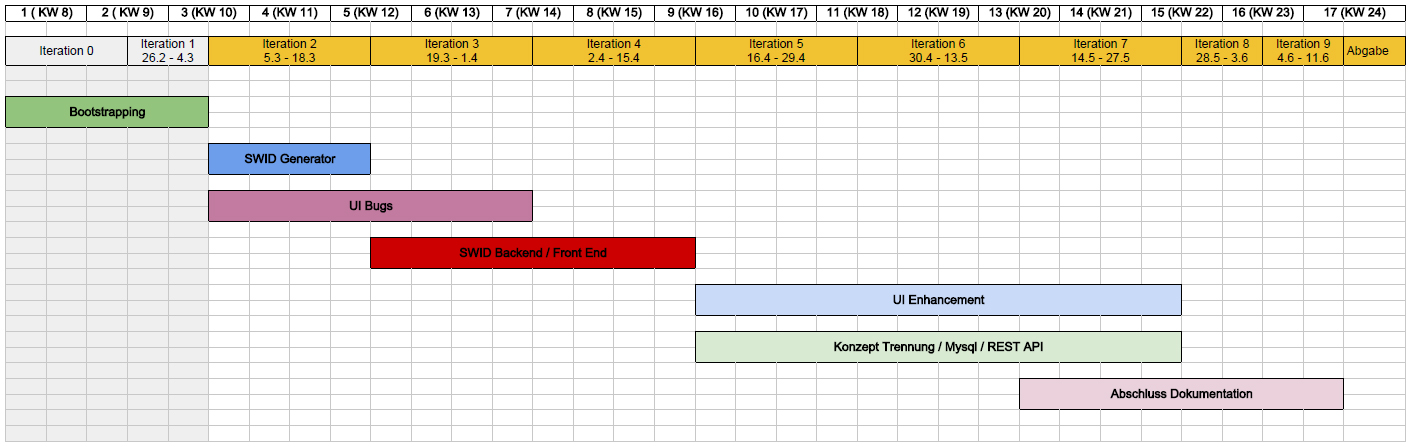
\includegraphics[width=\textwidth]{images/zeitplanung/Iteration1_2.jpg}
\subsection{Meeting 3 5.3.2014}
\paragraph{Status}
Eine initiale Planung wurde erstellt. Die Planung ist so ausgelegt, das als erstes die Pflichtteile erarbeitet werden sollen. Einerseits zur Risikominierung für uns und andererseits soll dadruch sichergestellt sein, dass die geforderte Funktionalität,  die Herr Steffen im Juni demonstrieren will, möglichst bald fertig ist und danach ausgiebig getestet werden kann und bis zur Präsentation einen möglichst stabilen Stand erreicht. Sobald diese Funktionalitäten erreicht sind, werden die optionalen Teile in einem separaten Fork integriert um die Stabilität weiterhin zu gewährleisten.
Das SQLite Schema wurde testweise auf MySql/Maria DB portiert. Dabei wurden einige Probleme festgestellt:
\begin{itemize}
\item Tabellennamen sowie Felder verwenden MySql Keywords wie Key/Keys
\item Es gibt Indizes über Felder des Types TEXT, das ist in Mysql so nicht möglich, eine einschränkung über deren länge ist nötig.
\item Die Referenzen in SQLite Syntax sind nur zur dokumentation vorhanden, sind aber leider etwas fehlerhaft. Es gibt verweise auf die nicht existente Tabelle measurements und einige Referenzen fehlen ganz. 
\end{itemize}

\paragraph{Zusammenfassung}

\begin{itemize}
\item Pflichtteile werden in der Planung priorisiert.
\item Die Migration auf MySQL wird nach hinten geschoben, da nicht pflicht und einige Probleme daraus resultieren könnten
\end{itemize}
\subsection{Meeting 4 12.3.2014}
\paragraph{Status}
Der Zeitplan konnte bisher eingehalten werden. Der Stand des SWID Generators konnte im Meeting vorgeführt werden, sieht soweit gut aus. 
Die File Tags sollen optional im output enthalten sein, um das Mapping von Files und Pakete zu erhalten. Dazu gibt es einen Use Case welchen wir im Frontend auch berücksichtigen sollten, siehe Todo. Wir haben noch lange über das Sequenzdiagramm diskutiert, es gibt es da noch einige Zuständigkeiten der einzelnen Komponenten, die noch nicht ganz klar sind. Wir werden das nächste Meeting das überarbeitete Diagramm nochmals mitbringen.

\paragraph{Zusammenfassung}
\begin{itemize}
\item Parameter für xml dokument separator (default: 2x newline)
\item Use gibt einen UseCase: File Hash stimmt nicht, aus welchem Pakage kommt das file?
\item Autodetection des Environments (dpkg/yum)
\item Deployment soll als executable vorliegen, dass zb mittels pip installiert werden kann
\item Nur installierte Packages auflisten, ist momentan noch nicht implementiert
\end{itemize}

\section{Iteration 3}
\subsection{Zeitplanung}
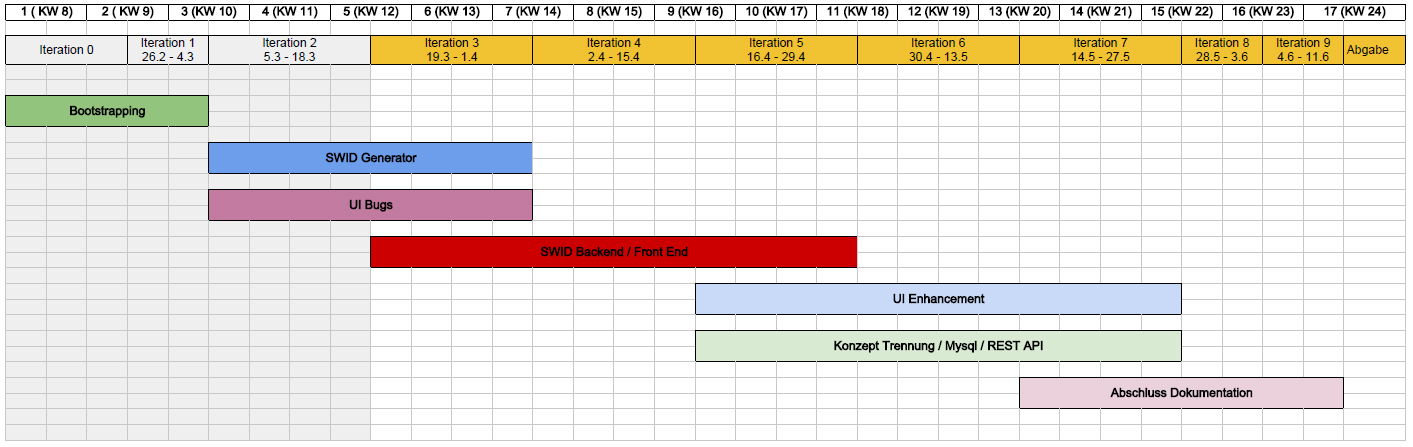
\includegraphics[width=\textwidth]{images/zeitplanung/Iteration3.jpg}
\subsection{Meeting 19.3.2014}
\paragraph{Status}

Wir liegen nicht ganz im Zeitplan, da Danilo zur Zeit noch im Spital ist. Entsprechend haben wir den Zeitplan angepasst und die Ziele etwas nach hinten in den vorgesehenen Puffer verschoben. Bis auf das File Listing konnten wir in dieser Iteration alle Ziele erreichen. Wir haben am Meeting eine erste Version des Datenmodells für die SWID Tag vorgestellt. Es gabe da einige Diskussionspunkte. Zum einen stellte sich die Frage ob wir die Daten in das bestehende Modell integrieren sollen oder komplett als Erweiterung (separate Tabellen). Folgende Punkte sind in der Diskussion aufgefallen
\begin{itemize}
\item XML String sollte RAW auch abgespeichert werden
\end{itemize}

\paragraph{Zusammenfassung}
\begin{itemize}
\item Readme für die SWID Generator Installation erstellen
\item Die Anforderungen ans Backend sind noch nicht sehr klar, wir beginnen mit erfassen von Use Cases, damit könnten sich viele Fragen zum Datenmodell beantworten lassen.
\item Blacklist Option im Package View ist überflüssig
\item Pull Request von aktuellem Stand (strongTNC) erstellen
\item Beim UI sollte bei der Suche bzw. Autocomplete auch die Option angeboten werden ein neues Item zu erstellen -> Usability
\end{itemize}

\subsection{Meeting 26.3.2014}
Die Meetings werden wir ab sofort wieder am Mittwoch morgen um 10:00 durchführen, damit wir den ganzen Nachmittag Zeit haben um gemeinsam zu arbeiten. Paketmanager liefern bei einer Abfragen nach enthalten Files in Paketen zum Teil Links auf Dateien die nicht existieren, und Ordner die nicht existieren, diese dürfen wir aber im File Payload dennoch mitliefern, da sie zum Paket gehören. Das Dropdownfeld im Policy View sollte zu einem Multiselect umgebaut werden, da mehrere Flags für eine Policy erlaubt sind. Die Architektur (64bit/32bit) sollte in die uniqueID aufgenommen werden, da es möglich ist, das 64bit Pakete aus anderen Dateien bestehen als die 32bit Versionen. Wir stellen das Vorgehen für Pull-Requests zurück zum Hauptrepository (strongTNC) um, sodass wir nicht mehr unseren master zurück "pullen" sondern jeweils einen eigenen Pull-branch erstellen welchen wir mittels Pull-Request in den strongTNC master pullen. Es gibt zur Zeit keine Funktion im GUI Files Einträge zu erstellen, das sollen wir noch ergänzen. Die bestehenden Use Cases sind soweit in Ordnung, während dem Meeting sind noch 2 sehr wichtige, bisher unbekannte Use-Cases dazugekommen: Generierung von Tag-ID's und die Targeted Requests nach SWID Tags.
Ein weiterer "nice-to-have" Use Case wäre Welches Tag gehört zu einem File. Ist aber explizit keine Muss Anforderung.
Da mit der CMDB Funktionälität der Stand eines Gerätes immer an einen bestimmten Zeitpunkt gebunden ist, sollen wir die Abfrage "Device-Report" so implementieren, dass z.B mittels Slider eine Datum oder Datumsbereich gewählt werden kann, für den der Status ersichtlich ist.

\section{Iteration 4}
\subsection{Zeitplanung}
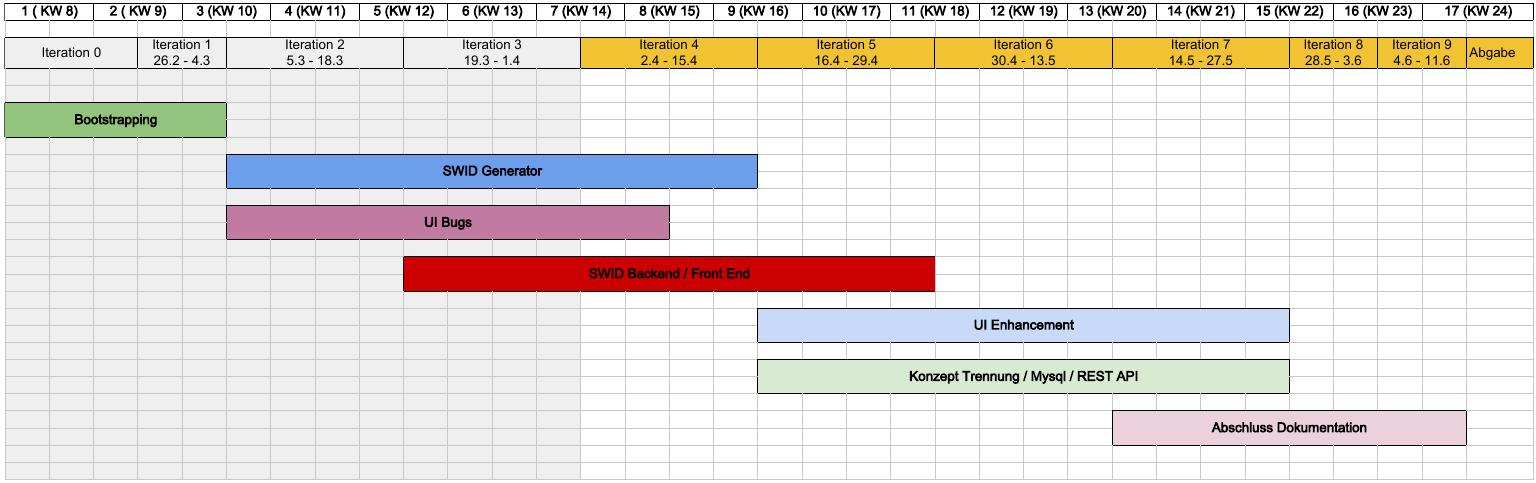
\includegraphics[width=\textwidth]{images/zeitplanung/Iteration4.jpg}
Die Phase für den SWID-Generator haben wir etwas verlängert, da letzte Woche noch 2 Use-Cases hinzugekommen sind.
\subsection{Meeting 2.4.2014}
Den zusätzlichen Use-Case für Software\_IDs haben wir unterdessen implementiert. Targeted Request müssen keine wildcards oder regex option anbieten, es gibt zur Zeit keinen Use-Case dafür. Es gab kurzfristig, vergangenen Montag, noch 2 Anpassungswünsche von Herrn Steffen: Zusätzliches Flag für IMA Messungen und  Sortierung der Sessions im Device Report absteigen (nach Datum). Wurde bereits implementiert und werden wir möglichst schnell in einem Pull-Request zur verfügung stellen.
Das Benutzerrollen Konzept ist so in Ordnung. Optimalerweise werden wir einen eigenen Decorator erstellen um redundaten code zu vermeiden. Im DB Modell ist noch eine kleine Anpassung notwendig, sodass mehrere Meassurmentreports für eine Session möglich sind. Das WSGI Script werden wir in den conf Ordner verschieben. Wir werden eine Deployment Anleitung für NGINX und Apache erstellen, wo wir auf die Änderung des WSGI Pfades hinweisen werden. 

\section{Iteration 5}
TODO
\section{Iteration 6}

\subsection{Zeitplanung}
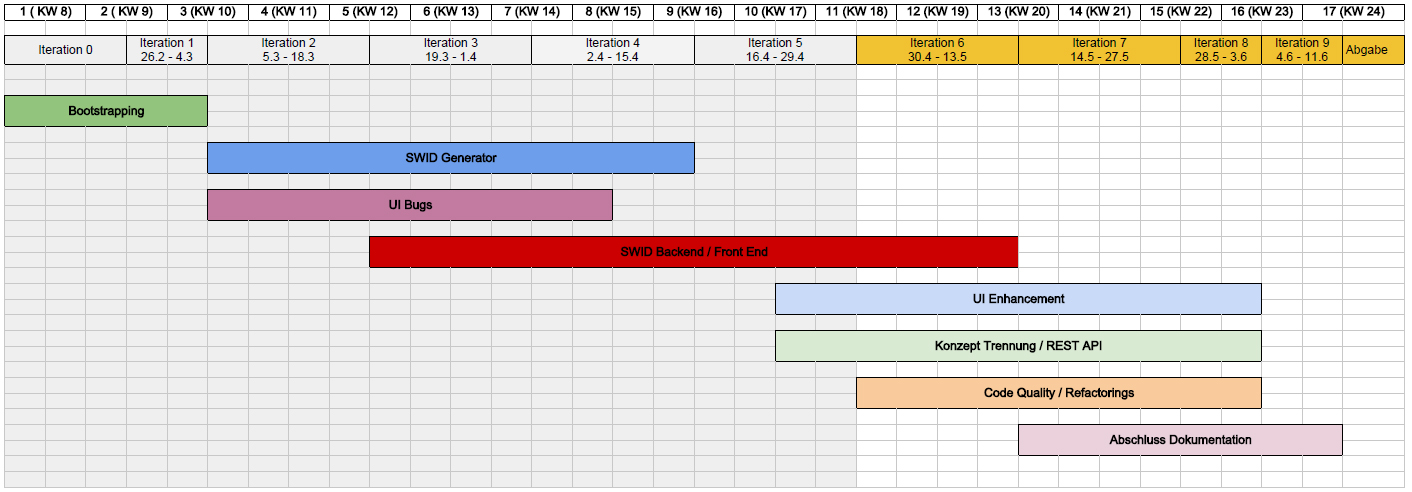
\includegraphics[width=\textwidth]{images/zeitplanung/Iteration6.jpg}

\subsubsection{Meeting 7.5.2014}
In der SWID Inventory View sollten wir Tags die durch die ausgewählte Sesssion hinzugekommen sind hervorheben. Das first reported Datum sollten wir zur jeweiligen Session verlinken. In der Session übersicht soll es mittels AJAX Paging möglich sein, nicht nur die letzten 50 Sessions anzuzeigen. Die erste Version des API Konzeptes sieht gut aus, Herr Steffen möchte es gerne als Proposale an die TCG senden, dazu werden wir das Konzept noch auf Englisch übersetzen. Im Anhang des Konzeptes werden wir noch ein paar CURL Beispiele zur programmatischen Benutzung der API auflisten. Die Präsentation der strongTNC Erweiterung wird am 25. Juni 2014 sein. In der Logview sollte der Diff (gelöschte Pakete / neue Pakete) angezeigt werden und der Zeitrahmen mittels Kalender eingestellt werden können. Der SWID Generator soll noch so erweitert werden, dass auch eine targeted Request nach Package name möglich ist (z.B OpenSSL), die Parameter sollen \texttt{---package} und \texttt{---software-id} sein. Ein grosser Mehrwert wäre das Matching von SWID Tags auf Packages, kann aber nicht mit 100\% Sicherheit gemacht werden. Das hätte den Vorteil, dass man sehen könnte welche Files für ein package geändert haben (z.B Security Patch) und könnte dann eine Messung auf diesen Files veranlassen.



